\documentclass{article}
\usepackage[utf8]{inputenc}
\usepackage[english]{babel}
\usepackage[font=small,labelfont=bf]{caption}
\usepackage{geometry}
\usepackage{natbib}
\usepackage{pxfonts}
\usepackage{graphicx}
\usepackage{newfloat}
\usepackage{setspace}
%\doublespacing


\title{How is experience transformed into memory?}
\author{Andrew C. Heusser, Paxton C. Fitzpatrick, and Jeremy R. Manning\\Department of Psychological and Brain Sciences\\Dartmouth College, Hanover, NH 03755, USA\\Corresponding author: jeremy.r.manning@dartmouth.edu}

\bibliographystyle{apa}

\begin{document}
\maketitle

\begin{abstract}
How our experiences unfold over time define unique \textit{trajectories} through the relevant representational spaces.  Within this geometric framework, one can compare the shape of the trajectory formed by an experience to that defined by our later remembering of that experience.  We propose a framework for mapping naturalistic experiences onto geometric spaces that characterize how they unfold over time.  New insights emerge when we apply this approach to a naturalistic memory experiment which had participants view and recount a video.  We found that the shapes of the trajectories formed by participants' recountings were all highly similar to that of the original video, but participants differed in the level of detail they remembered.  We also identified a network of brain structures that are sensitive to the ``shapes'' of our ongoing experiences, and an overlapping network that is sensitive to how we will later remember those experiences.
\end{abstract}


\section*{Introduction}

What does it mean to \textit{remember} something? In traditional episodic memory experiments \citep[e.g., list-learning or trial-based experiments;][]{Murd62a, Kaha96}, remembering is often cast as a discrete and binary operation: each studied item may be separated from the rest of one's experiences, and that item may be labeled as having been recalled versus forgotten. More nuanced studies might incorporate self-reported confidence measures as a proxy for memory strength, or ask participants to discriminate between ``recollecting'' the (contextual) details of an experience or having a general feeling of ``familiarity'' \citep{Yone02}. However, characterizing and evaluating memory in more realistic contexts (e.g., recounting a recent experience to a friend) is fundamentally different in at least three ways~\citep[also see][for a review]{KoriGold94}.  First, real world recall is continuous, rather than discrete.  Unlike in trial-based experiments, removing a (naturalistic) event from the context in which it occurs can substantially change its meaning.  Second, the specific words used to describe an experience have little bearing on whether the experience should be considered to have been ``remembered.''  Asking whether the rememberer has precisely reproduced a specific set of words to describe a given experience is nearly orthogonal to whether they were actually able to remember it.  In classic (e.g., list-learning) memory studies, precise recall is often a primary metric of assessing the quality of participants' memories.  Third, one might remember the \textit{gist} or essence of an experience but forget (or neglect to recount) particular details.  Capturing the gist of what happened is typically the main ``point'' of recounting a memory to a listener whereas, depending on the circumstances, accurate recall of any specific detail may be irrelevant.  There is no analog of the gist of an experience in most traditional memory experiments; rather we tend to assess participants' abilities to recover specific details (e.g., the precise stimuli they encountered earlier in the experiment).

How might one go about formally characterizing the gist of an experience?  Any given moment of an experience derives meaning from surrounding moments, as well as from longer-range temporal associations~\citep[e.g., ][]{LernEtal11}.  Therefore the timecourse of how an event unfolds is fundamental to its overall meaning.  Further, this hierarchy formed by our subjective experiences at different timescales defines a \textit{context} for each new moment~\citep[e.g., ][]{HowaKaha02, HowaEtal14}, and plays an important role in how we interpret that moment and remember it later~\citep[for review see][]{MannEtal15}.  Our memory systems can then leverage these associations to form predictions that help guide our behaviors~\citep{RangRitc12}.  For example, as we navigate the world, the features of our subjective experiences tend to change gradually (e.g.\ the room or situation we are in is strongly temporally autocorrelated), allowing us to form stable estimates of our current situation and behave accordingly~\citep{ZackEtal07, ZwaaRadv98}.  Although our experiences most often change gradually, they also occasionally change suddenly~\citep[e.g., when we walk through a doorway; ][]{RadvZack17}.  Prior research suggests that these sharp transitions (termed \textit{event boundaries}) during an experience help to discretize our experiences into \textit{events}~\citep{RadvZack17, BrunEtal18, HeusEtal18, ClewDava17, EzzyDava11, DuBrDava13}.  The interplay between the stable (within event) and transient (across event) temporal dynamics of an experience also provides a potential framework for transforming experiences into memories that distill those experiences down to their essence-- i.e., their gists.  For example, prior work has shown that event boundaries can influence how we learn sequences of items~\citep{HeusEtal18, DuBrDava13}, navigate~\citep{BrunEtal18}, and remember and understand narratives~\citep{ZwaaRadv98, EzzyDava11}.

Here we sought to examine how the temporal dynamics of a ``naturalistic'' experience were reflected in participants' later memories of that experience.  We analyzed an open dataset which comprised behavioral and functional Magnetic Resonance Imaging (fMRI) data collected as participants viewed and then verbally recalled an episode of the BBC television series \textit{Sherlock}~\citep{ChenEtal17}.  We developed a computational framework for characterizing the temporal dynamics of the moment-by-moment content of the episode (and of participants' verbal recalls).  Specifically, we use topic modeling~\citep{BleiEtal03} to characterize the thematic conceptual (semantic) content present in each moment of the episode and recalls, and we use Hidden Markov Models~\citep{Rabi89, BaldEtal17} to discretize the evolving semantic content into events.  In this way, we cast naturalistic experiences (and recalls of those experiences) as \textit{topic trajectories} that describe how the experiences evolve over time.  In other words, the episode's topic trajectory is a formalization of its gist.  Under this framework, successful remembering entails verbally ``traversing'' the topic trajectory of the original episode, thereby reproducing the gist of the original episode.  In addition, comparing the shapes of the topic trajectories of the original episode and of participants' retellings of the episode reveals which aspects of the episode were preserved (or lost) in the translation into memory.  We also identified a network of brain structures whose responses (as participants watched the episode) reflected the gist of the episode, and a second network whose responses reflected how participants would later recount the episode.


\section*{Results}
To characterize the gists of the \textit{Sherlock} episode participants watched and their subsequent recountings of the episode, we used a topic model~\cite{BleiEtal03} to discover the latent thematic content.  \cite{ChenEtal17} collected hand-annotated information about each of 1000 (manually identified) scenes spanning the roughly 45 minute video.  This information included: a brief narrative description of what was happening; whether the scene took place indoors vs. outdoors; names of any characters on the screen; names of any characters who were in focus in the camera show; names of characters who were speaking; the location where the scene took place; the camera angle (close up, medium, long, etc.); whether or not background music was present; and other similar details (for a full list of annoted features see \textit{Methods}).  We took from these annotations the union of all unique words (excluding stop words, such as ``and,'' ``or,'' ``but,'' etc.) across all features and scenes as the ``vocabulary'' for the topic model.  We then concatenated the sets of words across all features contained in overlapping 50-scene sliding windows, and treated each 50-scene sequence as a single ``document'' for the purposes of fitting the topic model.  Next, we fit a topic model with (up to) $K = 100$ topics to this collection of documents.  We found that 28 unique topics were sufficient to describe the time-varying content of the movie (see \textit{Methods}).  Note that our approach is similar in some respects to Dynamic Topic Models~\citep{BleiLaff06}, in that we sought to characterize how the thematic content of the data evolved over time.

\begin{figure}[tp]
\centering
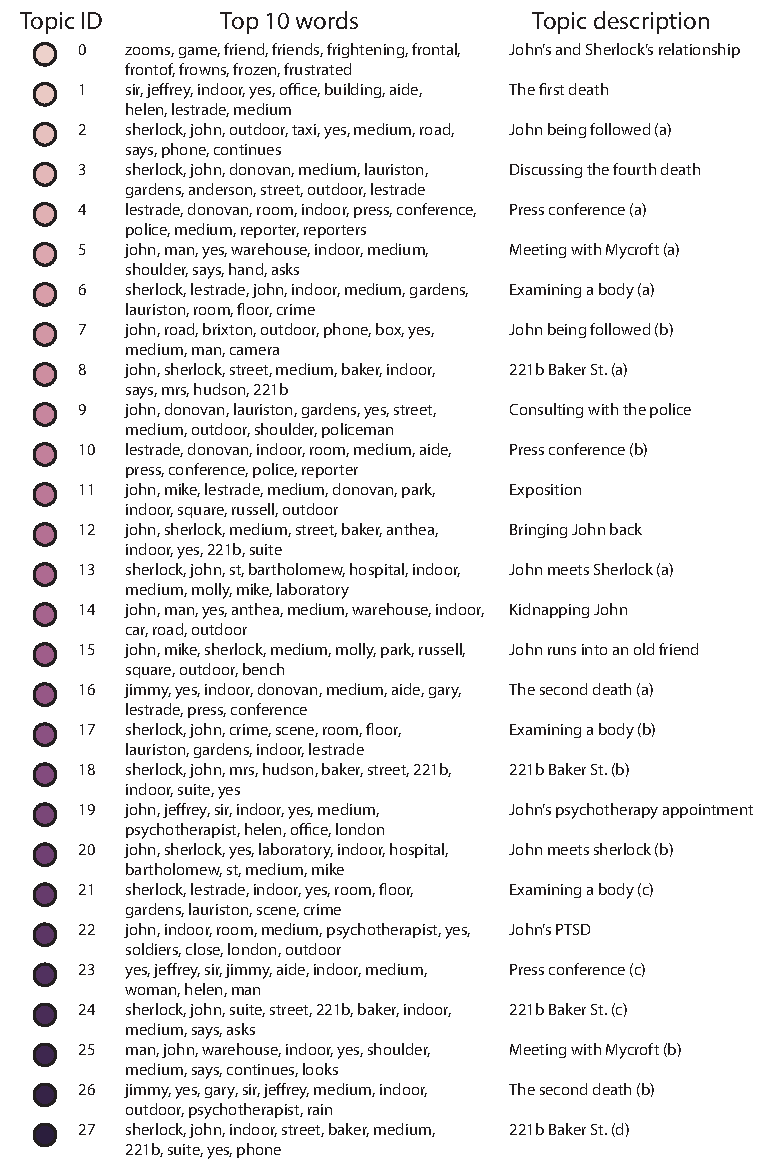
\includegraphics[width=0.5\textwidth]{figs/0_topics.pdf}
\caption{\small \textbf{Topics discovered in \textit{Sherlock}.} We applied a topic model to hand-annotated information about 1000 scenes spanning the 45 minute episode.  We identified 28 unique topics with non-zero weights (we used $K=100$ topics to fit the model).  Each topic comprises a distribution of weights over all words in the vocabulary.  For each topic, we show the words with the 10 largest weights, along with a suggested description of the topic.}
\label{fig:topics}
\end{figure}

The topics we found appeared heavily character-focused (e.g. the top-weighted word in each topic was nearly always a character) and could be roughly divided into themes related to primarily Sherlock-focused; primarily (John) Watson-focused (Watson is Sherlock's close confidant and assistant); and themes that involved Sherlock and Watson interacting (Fig.~\ref{fig:topics}).  Several of the topics also appeared highly similar, which we hypothesized might allow us to distinguish between subtle narrative differences (e.g., if the distinctions between those overlapping topics were meaningful), but could also impair characterization of the narrative (e.g., if the distinctions between topics were not meaningful).

%JRM STOPPED HERE

% characterize gist of movie and recalls
% 1. movie: fit topic models (add note on dynamic topic models).  fig 1: what do the topics reflect (top words from each topic), example with a few scenes.
% 2. notice block diagonal structure, rather than smooth transitions; motivates HMM approach.  Note about selecting K
% 3. question: do recalls exhibit same structure?  apply topic model to recalls.  note that by projecting everything into a common topic space, the thematic content of each moment of movie/recall can be compared, even though the mix of words used to describe any given event or moment may not be consistent across people (or across annotations/recall)
% 4. recalls exhibit blocky structure, but at different scales.  motivates fitting K separately by person
% 5. match up events (correlations)
% 6. now we can use classic memory analyses to examine structure of recall.  motivate and reference PFR, lag-CRP, and SPC.  but this does not tell us about structure in the *content* of what people remembered, or whether people's recalls are capturing the hierarchical temporal structure of the original movie.
% 7. topic trajectories as a new way of characterizing recall.  assess agreement using rayleigh test.  also examine shapes of each subject's trajectory to show match.  key insight: everyone captures the general shape, but at different "sampling resolutions"
% 8. we can also project back onto the original (word) features to understand more about what any particular part of the trajectory reflects (wordle fig)
% 9. the above analyses tell us about how the trajectory of thematic content in the episode is both preserved and transformed in participants' memories.  we next carried out analyses to understand the neural bases of these phenomena.  analysis 1: which structures are sensitive (during viewing) to the original episode's topic trajectory?  answer: default mode.  anlaysis 2: which structure are sensitive (during viewing) to how the participants will later recall the episode?  answer: vmPFC, default mode.  (potential role of vmPFC in reflecting participant-specific memory transformations and processing)



We sought to formalize the gists of a naturalistic stimulus (an episode of the \textit{Sherlock} television show) and participants' recountings of that stimulus.
% JRM STOPPED HERE
% - add a general overview
% - some of this seems like it belongs in methods...
% - possible section title change to "Narrative?" -- see author guidelines and prior nature submissions


\begin{figure}[tp]
\centering
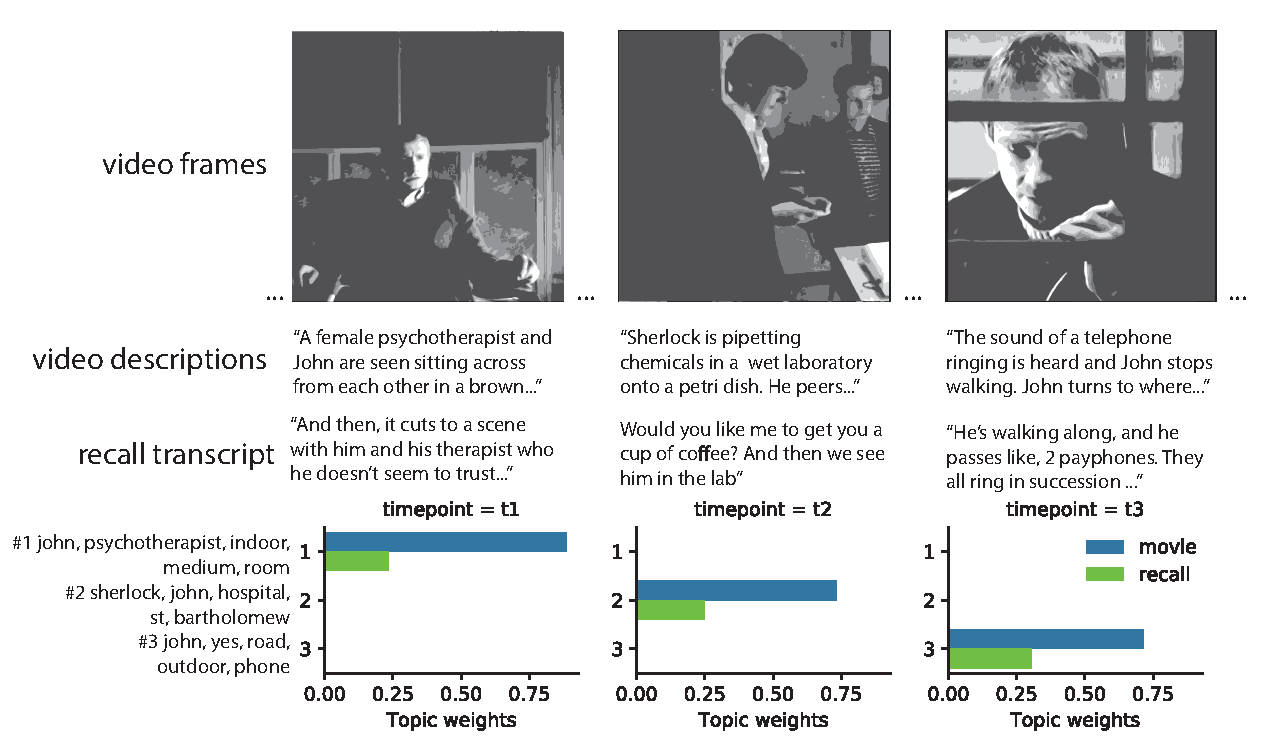
\includegraphics[width=1\textwidth]{figs/1_analysis_schematic_bw.pdf}
\caption{\small \textbf{Schematic of the analysis approach.} For each scene in the video, text descriptions were generated by hand. Three exemplary time points are displayed here.  Below the video descriptions are text samples from an example participant's verbal recall transcript.  We fit a topic model to the moment-by-moment video text descriptions and transformed participants' verbal recall transcripts using this same model. The bar charts display the resulting topic model weights for the video (in blue) and recall (in green) for three example topic dimensions.}
\label{fig:schematic}
\end{figure}

\subsection*{Modeling the naturalistic stimulus and verbal recall}
We fit a topic model \citep{BleiEtal03} to hand-annotated text descriptions of scenes from the video. The text descriptions contained details of the scene such as the characters present, location, and a short summary of the scene (see Fig.~\ref{fig:schematic} for example text). As depicted in Fig.~\ref{fig:model}A, the topic vectors are sparse and change slowly over time. Furthermore, there are clear transitions from one topic ``state'' to the next, possibly indexing scene transitions in the stimulus. To get a better handle on this temporal structure, we computed a timepoints (1976) by timepoints (1976) correlation matrix of the video model (Fig.~\ref{fig:model}C).  This correlation matrix reveals that the model has a strong, block-diagonal structure with very low off-diagonal correlation values, suggesting the representations of each block are unique and highly discriminable. We found that the ``narrative details'' (a few sentences summarizing the dialogue and specific happenings of the scene) of the video were the most important feature driving this model structure (see Fig.~S3A).

After watching the video, participants verbally recalled (in order) as much of the episode as they could.  We used the same topic model (fit with the text descriptions of the video) to transform participants' verbal recall transcripts. An example participant's (\#13) recall model is plotted in Fig.~\ref{fig:model}B. Notably, participant \#13's recall model appears visually similar to the video model. Similar to the video model analysis (Fig.~S3A), we found that the ``narrative details'' feature was most important for driving the video/recall relationship (Fig.~S3B).  Like the video model, topic vectors were sparse and changed gradually.  Then, we investigated the temporal structure of the recall matrices. From each participant's recall model, we computed a sentences (68 to 294) by sentences (68 to 294) correlation matrix (Fig.~\ref{fig:model}D). Like the video model, each participant's recall correlation matrix exhibited a strong block-diagonal structure (Fig.~S1). Notably, this suggests that participants recounted the video in discriminable segments, likely related to the recall of specific events from the video.


\begin{figure}[tp]
\centering
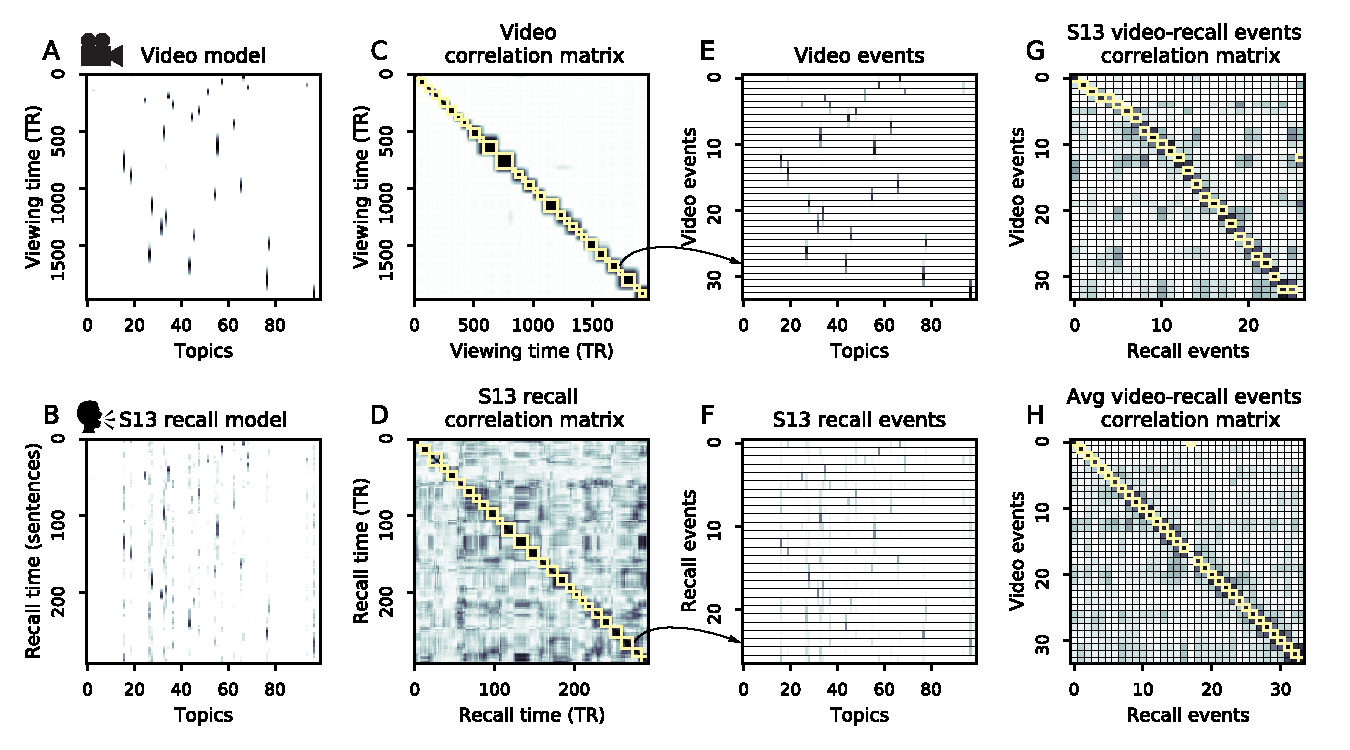
\includegraphics[width=\textwidth]{figs/2_eventseg.pdf}
\caption{\small \textbf{Modelling naturalistic stimuli and recall.} A depiction of our analysis pipeline. For all plots, darker colors indicate greater values and the range of each plot is 0-1.  \textbf{A.} A timepoints (1976) by topics (100) matrix representing the video stimulus.  Each row represents the most likely mixture of topics for a given timepoint (i.e., topic weights). Each column represents a different topic. \textbf{B.} A sentences (294) by topics (100) matrix representing participant \#13's recall. \textbf{C.} A viewing-time (1976) by viewing-time (1976) correlation matrix representing the correlation of each moment of the video model with every other moment of the video model. The yellow boxes represent `events' recovered by a hidden Markov model. \textbf{D.} A recall-time (294 sentences) by recall-time (294) correlation matrix for participant \#13. \textbf{E.} An events (34) by topics (100) matrix where each row represents the average topic vector for each event in the video model.  \textbf{F.} An events (27) by topics (100) matrix where each row represents the average topic vector for each event in participant \#13's recall model. \textbf{G.} A recall events (27) by video events (34) correlation matrix for participant \#13. The cells with a yellow border identify the video event with the highest correlation to a given recall event. \textbf{H.} A group averaged recall events (34) by video events (34) correlation matrix.  The cells with yellow borders are the video event with the highest correlation to a given average recall event.}
\label{fig:model}
\end{figure}

\subsection*{Segmenting the video and recall models into ``events''}
As described above, a striking feature of both the video and recall correlation matrices is a strong, block structure along the diagonal of the matrices (see Fig.~\ref{fig:model}C,D).  We hypothesized that this structure might arise from transient stability in the "theme" of both the video and of participants' memory for the video. We hypothesized that specific events described by a participant could be ``matched'' to specific video events by computing the similarity (i.e., correlation) between their topic vectors. In other words, the video event that is most thematically similar to a particular recall event is the event that the participant is most likely describing. To test this idea, we segmented the video and recall models in $k$ events (i.e., states) using a hidden Markov model ~\citep{BaldEtal17}. Our algorithm determined 34 events for the video model and a range of values (range: 8-27; mean: 15.41; SD: 5.6) for the recall models (see Methods for details on choosing an optimal $k$ value).  The events discovered for the video model and a representative participant's recall model are highlighted as yellow rectangles outlining blocks along the diagonal of the correlation matrices (Fig.~\ref{fig:model}C,D).

Next, we created a video ``event model'' by averaging together neighboring topic vectors that the were classified to be in the same event, resulting in an events (34) by topics (100) matrix (Fig.~\ref{fig:model}E).  We performed the same procedure for the recall matrices (Fig.~\ref{fig:model}F). Then, we computed the correlation between video and recall event models, resulting in a video events (34) by recall events (8-27, depending on the participant) correlation matrix (Fig~\ref{fig:model}G for example, Fig.~S2 for all participants). These matrices represent the similarity (correlation) between each video event and each recall event (for each participant). To determine which video event a particular recall event was most likely describing, we found the index of the video event with the highest correlation to the recall event (i.e., the argmax).  This is depicted in Fig.~\ref{fig:model}G as the cells highlighted with a yellow border. Notably, our algorithm suggests that the example participant recalled most of the video events and did so in order.

Then, we computed a group-averaged recall event model and video-recall event correlation matrix. For each participant (and each recall event), we sorted the recall event vectors (across all participants) according to the video event with the highest correlation. We then averaged the recall event vectors within each group. This yielded an average recall event vector for all but one (of 34) video events, since no participant remembered one of the events according to our model. Lastly, we computed an average recall event (34) by video event (34) correlation matrix, and highlighted the cell with the highest correlation value with a yellow border (Fig.~\ref{fig:model}H). Notably, this matrix displayed high correlation values along the diagonal and low correlations in the off-diagonal cells. This suggests that on average, participants were able to recapitulate the events in the episode in a specific, sequential and highly descriminable way.

\subsection*{The trajectory of a naturalistic experience is preserved in recall}
Classic approaches to studying free recall in episodic memory (such as overall accuracy and serial position curve) focus on the quantity of information recalled \citep{Murd62a}. More recent metrics (such as lag-CRP, semantic and temporal clustering) go further to describe list-level memory organization \citep{Kaha96, PolyEtal09}. However, these approaches cannot (and were not designed to) capture the rich temporal dynamics inherent in naturalistic stimuli and associated recall of those experiences. In the next set of analyses, we test the hypothesis that successful recall of a naturalistic stimulus entails recovering the trajectory of a stimulus.

\begin{figure}[tp]
\centering
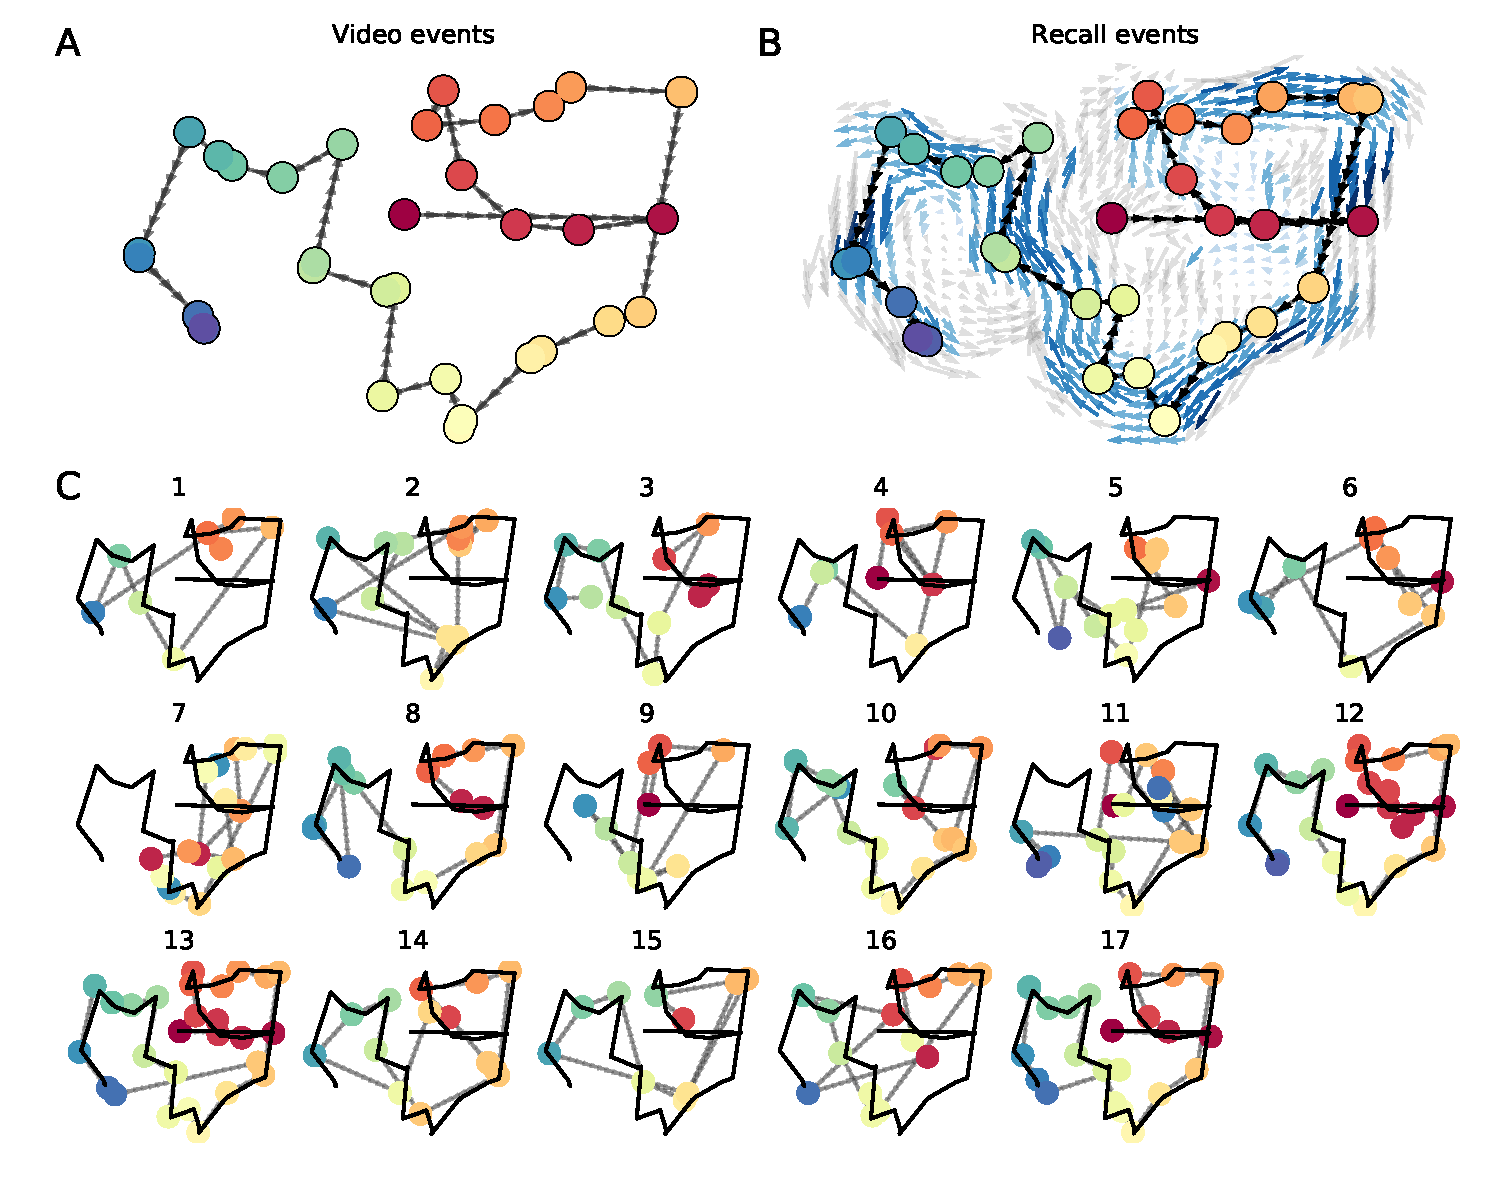
\includegraphics[width=1\textwidth]{figs/3_trajectory.pdf}
\caption{\small \textbf{Video and recall trajectory plots.} \textbf{A.} 2-dimensional embedding of the video events model (reduced with UMAP algorithm). The arrows indicate the forward direction of the video events. \textbf{B.} 2-dimensional embedding of the average recall events model.  The colors refer to the most similar video events. The directional lines connecting the points represent the true video event order. The arrows represent the group-average direction of all recall event transitions (i.e., a line segment connecting two consecutive recall event vectors) that intersected a circle (radius = 0.5) centered on the origin of the arrow. \textbf{C.} Individual trajectory plots for each participant overlayed with the video model (black). The direction of the recall sequence is indicated by the direction of arrows connecting each recall event.  The colors refer to the most likely video event.}
\label{fig:trajectory}
\end{figure}

To visualize the relationship between the video and recall event models, we embedded them into a 2D space using the UMAP dimensionality reduction algorithm ~\citep{McInHeal18}, where the points represent video/recall events and the distance between them represents their similarity/distance in ``topic space'' (Fig.~\ref{fig:trajectory}A).  We observed that visually, it appears that the two models have a very similar temporal evolution and geometric structure. To further quantify this correspondence and to characterize how participants navigated through the space during recall, we analyzed the angle between successive recall events. We created a grid of evenly spaced points (.25 units) in the 2D ``topic space.'' For each point on the grid, we drew a circle (radius= 0.5) around the point and grouped together all recall transitions that intersected the circle (across participants). To visualize the average angle, we converted each transition angle to a unit vector and then averaged the vectors together. To assess consistency in the direction of the recall transition across participants, we performed a Rayleigh test ($p < 0.001$, corrected at $p < 0.05$ using the permutation procedure described in Methods). Notably, the video events fell within the path formed by the recall events.  Thus, participants' recalls followed the same path as the video model (Fig.~\ref{fig:trajectory}B), suggesting the shape of the stimulus was preserved despite idiosyncratic differences between participants in their recalls.

%NOTE: it feels like we need some more supporting evidence that the shape of the video and the recall trajectories are related.  one possibility would be to add the analysis where i compute the distance between each recall event and the line formed by each video transition per participant. the result is that hand annotated memory correlates to this distance, suggesting that participants who better capture the shape also have better memory on average.

\subsection*{Brain regions that mirror the correlational structure of naturalistic stimuli and memories}.
\begin{figure}[tp]
\centering
\includegraphics[width=1\textwidth]{figs/4_brains_panels.pdf}
\caption{\small \textbf{Video and recall model correlational structure searchlight analysis.} \textbf{A.} The correlation matrix representing the temporal structure of the video model. Below it is a surface plot of brain regions whose activity patterns mirrored the correlational structure of video model during viewing.  \textbf{B.} The left matrix is S13's video-recall correlation matrix before warping. The yellow stars represent the path recovered by dynamic time warping. The right matrix is the result after warping. The same warping path was applied to the fMRI timeseries (separately for each participant). A surface plot of brain regions whose activity patterns mirrored the participant-specific recall correlation matrix. Significance threshold (p$<$.05) for both video and recall analyses derived from a permutation procedure by phase shifting the video model and recomputing the z-scores.}
\label{fig:brainz}
\end{figure}

Previous work suggests that the brain may represent our experiences as ``events'' with different time scales in a nested hierarchy ~\citep{LernEtal11, ChenEtal17, BaldEtal17}. In this next analysis we asked: what brain regions mirror the event-like correlational structure of our topic-based video model during viewing? We used a searchlight procedure (see Methods for details) to identify regions whose timepoint-by-timepoint correlational structure matched the correlational structure of our model. This analysis revealed a network of regions including bilateral frontal and cingulate cortex (Fig.~\ref{fig:brainz}), suggesting that these regions may play a role in maintaining information relevant to the narrative trajectory of the video.

While each participant remembered roughly the same sequence of events, there were subtle idiosyncracies in the way each individual described the events. For example, the event-by-event similarity structure (i.e., the off-diagonal values of the recall correlation matrices) differed across individuals (Fig.~S1). We hypothesized that idiosyncracies in the recall dynamics across participants might be related to the temporal structure of brain networks representing the events during video viewing. In this analysis, we identified brain areas whose responses at the time of viewing exhibited the same (segmented) idiosyncratic dynamics that later appeared in that participants’ recalls. Using a procedure similar to the approach above (see Methods for details), we searched for regions whose correlational structure during viewing was related to the idiosyncratic structure of the participant's recall model. The resulting map suggests that the correlational structure of a network of brain regions including the ventromedial prefrontal cortex, anterior cingulate, and right medial temporal lobe mirror the idiosyncratic structure of participants' recalls (Fig.~\ref{fig:brainz}).

\begin{figure}[tp]
\centering
\includegraphics[width=1\textwidth]{figs/5_topics.pdf}
\caption{\small \textbf{Analysis of topics by event memorability.} \textbf{A.} Group-averaged correlation between each video event and closest recall event. Error bars represent 95\% confidence intervals. Stars indicate top (green) and bottom (red) 3 remembered events across participants \textbf{B.} Wordles (top 200 words) representing a weighted average of video event topic vectors weighted by event memorability (e.g., the correlation values in A). The top wordle (green) contains words from the most remembered events and the bottom (red) contains words from least memorable events. The word sizes are proportional to the word's ``activation''. \textbf{C.} Trajectory represents the video event model embedded in a 2D space using UMAP. The large colored dots are video events. The small colored dots are individual recall events across all participants, where the colors correspond to the closest video event. The circular wordles represent the top 3 most (green circles) and least (red) memorable video events.  The left side of the wordle circles contain words associated with the video event vector and the right side contains words associated with the average recall event vector.}
\label{fig:topics}
\end{figure}

\subsection*{Memorability by event and topics}
A notable advantage of representing naturalistic stimuli and memory using this approach is that the event models can be mapped back to the language used to fit the model(s).  This allows for analysis (and visualization) of the language used when participants recounted their experiences.  In this next analysis, we 1) quantified the memorability of each video event and 2) used memorability to plot the ``top'' words for the most and least memorable scenes.

To measure video event memorability, we computed the correlation between each video event and the closest recall event and then averaged those values within participants (Fig.~\ref{fig:topics}A). We used event memorability to create a weighted average over all video event vectors, where video events with better memory were weighted more heavily. Then, we extracted the top 200 words and created ``wordles'' representing the most memorable themes in the video. The results reveal that scenes containing ``Sherlock'' and ``John'' were highly memorable, as were scenes containing words such as ``medium'', ``street'' and ``baker'' (Fig.~\ref{fig:topics}B). To find words related to the least memorable scenes, we inverted the memorability weights and again extracted the top 200 words.  Scenes containing ``Mike'' and ``Molly'' were least remembered, and also words like ``conference'', ``hospital'' and ``psychotherapist'' (Fig.~\ref{fig:topics}B).

Then, we took a closer look at the themes contained in the top/bottom 3 events, using the memorability weights to select the top/bottom events. We performed the same analysis as described above, but separately for the video and average recall event vectors representing each of the top/bottom 3 remembered events. In Figure~\ref{fig:topics}C, the trajectory represents a low-dimensional embedding of the video model and the large colored dots represent the video events. The smaller colored dots represent the distribution of individual recall events across all participants, colored by the closest video event. We plotted wordles for the top 3 (circled in green) and bottom 3 (red) most/least remembered events, where the video is represented in the left half of the circle and the average recall is represented in the right half of the circle. Visual inspection reveals that the words contained in the memorability weighted worldles (Fig.~\ref{fig:topics}B) overlap with the individual top/bottom event wordles (Fig.~\ref{fig:topics}C). These analyses shed light on the contents of naturalistic stimuli and accompanying memories, and highlight the flexibility in transforming between human and machine readable representations of the data afforded by our modeling approach.

\subsection*{Additional measures of naturalistic recall}
Representing the video and verbal recall as events in ``topic space'' also affords us the ability to characterize the quality of recall in a more fine-grained and nuanced way than was previously possible. We quantified the distance between each video event and its matching recall event (``precision''), the the distance between a video event and all non-matching recall events (``distinctiveness'') and the temporal order of the recall events (``order''). All three of these metrics were correlated to hand-annotated memory performance across participants ($p < 0.05$, see Supplemental Materials Section 1 for details).

Just like in a traditional free recall list-learning experiment where participants view a list of words and then verbally recall them, our video-recall matching analysis approach affords us the ability to analyze memory in the same way. We considered 6 classic list-learning analyses: overall accuracy, probability of first recall \citep{Hoga75, HowaKaha99, Lami99}, lag-conditional response probability \citep{Kaha96, HowaKaha99}, serial position curve \citep{Murd62a}, temporal clustering, and semantic clustering \citep{HowaKaha02, PolyEtal09}. Extending these classic list-learning analyses to naturalistic stimuli allows to directly compare trial- and naturalistic-based recall studies (see Supplemental Materials Section 2 for details).

\section*{Discussion}
\label{sec:discussion}
Studying human memory is commonly distilled down to a process of matching specific moments of a past experience with specific mnemonic outcomes.  In traditional trial-based free recall experiments, individual stimuli encountered during encoding are typically labeled as ``remembered'' or ``forgotten'' depending on whether the stimulus is recalled/recognized during a subsequent test. While this approach has advanced our understanding of human memory immensely, it does not translate well to naturalistic experiences. For one thing, the contents of our recall at any given moment might be reflected in many prior experiences/moments. Furthermore, the particular words used to describe the experience will inevitably vary across people and even across repeated recollections within an individual. Thus, there is not a ``one-to-one'' mapping between naturalistic experiences and their mnemonic counterparts. For example, remembering the patterns and colors of each person's shirt in a crowd might be considered as excellent recall in a standard memory task setup. But if the rememberer failed to note that the people in the crowd were gathered for their surprise birthday party, then they would have missed the "point" of the experience.

Our topic modeling approach, whereby we consider the broad ``theme'' present in different moments of participants' experiences and their memories for those experiences, affords us the ability to flexibly and accurately characterize memory for naturalistic experiences. This approach allows us to quantify which moments from the past and the current recounted experience match in terms of their thematic content and critically, our ability to perform this matching does not require participants to use any specific overlapping words. Our work characterizes recollection of an experience by comparing the overall ``shape'' of a dynamic stimulus and a memory. We assess the quality of memory for the video participants viewed by measuring the match between the shapes of the video's trajectory and each participant's recall trajectory. By contrast, the number of recalls could be captured by the "sampling frequency" along that trajectory -- but the number of recalls alone cannot tell us whether participants successfully recollected the meaning of the story by capturing the salient points of the narrative that define its main shape. In addition to providing a way to capture the shape of an experience, this method affords the ability to quantify the particular contents of memory.  Whereas traditional approaches abstract over the content (e.g., percent correct), Our approach allows one to quantify which aspects of an experience are memorable and which fail to stick. This aspect of our approach opens the door for a much richer characterization of memory that considers not just how much information was recalled, but the particular details of that information as well.

Prior work on neural responses during naturalistic experiences and recall has largely focused on identifying brain regions whose responses are reliably similar across individuals ~\citep{LernEtal11, SimoEtal16, ChenEtal17, BaldEtal17, ZadbEtal17}. This allows one to identify which regions might be processing or representing the stimulus, or retrieving details of the experience during recall. Our approach is fundamentally different. We ask: which brain regions during video viewing match the video structure and how individual participants will recall the video later (in terms of the temporal correlations of their recall topic trajectory)? This latter approach highlights regions such as the medial prefrontal cortex (mPFC) and medial temporal lobes (MTL) that may respond in idiosyncratic ways across individuals, but that nonetheless play an important role in encoding experience into memory. In other work, the mPFC has been suggested to play a role in the representation of a ``schema'', or a network of prior knowledge that is consistent with the current task ~\citep{KestEtal12, GilbMarl17}. One interpretation for mPFC's involvement in our work is that mPFC represents participant-specific relationships with the content of the video, and its representation during scene viewing is related to how a participant later describes the scene. MTL activity patterns also matched participant's recall, which is consistent with a large body of literature highlighting the role of the MTL in episodic memory encoding ~\citep{PallWagn02, DavaEtAl03, RangEtal04, Dava06}.

More broadly, these findings have strong implications for how we assess memory in other naturalistic contexts, such as the classroom or in a doctor's office.  Whereas academic tests often measure students' performance using metrics such as the proportion of correctly answered questions, our work suggests that this approach might ``miss the forrest for the trees''. We view ``true learning'' as understanding key concepts (i.e., understanding central themes in the learned content and how they relate) rather than regurgitating the greatest number of facts. In addition to educational contexts, our approach may provide unique metrics that can be used to assist in the diagnosis of memory disorders, and other psychiatric disorders that influence memory. For example, while the quantity of information recalled could be roughly matched between a healthy and patient population, and other aspects of the memory (such as the shape, serial order, precision or distinctiveness) might be different. Thus, this work serves as a foundation for more nuanced approaches to memory assessment that consider the trajectory and specific contents of memory for a naturalistic experience.

An important question for future work concerns the factors that drive an individual to sample their recall trajectory finely or coarsely. For example, given a short recall interval, would participants intuitively gravitate towards coarser samplings that still outline the basic shape of the video's topic trajectory? Or if participants were told that their narrations would be played back to other participants ~\citep{ZadbEtal17}, would that change the resolution or shape of their recalls? And over successive recountings of the same sequence of events or with more elapsed time between encoding and recall, how do the shapes of the trajectories change? For example, loss of detail would result in a "smoothing out" of the trajectories with each new retelling.

While we view this work as a major advance in characterizing and understanding human memory, as with any approach there are limitations. First, the approach relies on having a ``good'' model of the stimulus (e.g., one that describes the video in the same way as participants recall it), which is currently only achievable by a human hand-annotating each moment of the video.  To increase the scalability of this approach, future work could explore automated methods for extracting meaning from videos ~\citep{YuEtal16}.  Another potential limitation is that by its nature, the model extracts the ``gist'' of scenes from the video.  This provides desirable flexibility (e.g., participants can use different combinations of words to describe the scenes), but this comes at the expense of capturing specific details.  Thus, a future direction of this work will be to increase sensitivity to such details while maintaining flexibility.

To conclude, we'll revisit the question of what it means to remember something. Our view is that ``successful remembering'' is about recovering the ``trajectory'' of an experience, rather than the ability to recognize/recall any of its particular isolated details. Decades of research suggest that episodic memories are not veridical and context-free snapshots of the past, and so treating (and modelling) them as such is overly simplistic at best (and counterproductive at worst). While it's undeniable that these models have been useful in advancing our understanding of human memory, they are severely limited in their ability to explain memory for real life experiences. Real life experiences are highly structured in time, and so to have a complete understanding of the human memory system, our experiments and models of memory must not ignore this fact. Our work provides a theoretical advance in our understanding of what it means to remember as well as a novel methodological tool to study it.

\section*{Methods}
\label{sec:methods}

\subsection*{Participants and Experimental Design}
Participants ($n=17$) viewed the first 50 minutes of ``A Study in Pink'', an episode of the BBC series, \textit{Sherlock}. Immediately upon completion of the video, participants were instructed to (verbally) recount the events in the \textit{Sherlock} episode in their original order and in as much detail as possible. During the entire experiment, participants were in an fMRI scanner. For comprehensive details of the experimental procedures, please refer to \cite{ChenEtal17}.
%NOTE: is this sufficient or should i provide more detail?

\subsection*{Fitting the topic model to the video text and recall transcripts}
A topic model was used to estimate the most likely mixture of topics for a given sample of text. First, the video was manually segmented into 1000 scenes, and a collection of descriptive features was manually transcribed. For each scene, we considered the following features: narrative details (a sentence or two describing what happened in that scene), whether the scene was indoor or outdoor, name of all the characters in the scene, name of the character in focus, name of the character speaking, location, camera angle, music presence, and text on the screen. We concatenated the text for all of these features within each segment, creating a ``bag of words'' describing each scene. We then transformed the text descriptions into overlapping windows of 50 scene segments. For example, the first text sample comprised the text from the first 50 segments, the 2nd comprised the text from n+1:n+51, and so on. We trained our model using these overlapping text samples with scikit-learn's (version 0.19.1) `CountVectorizer' and `LatentDirichletAllocation' classes \citep{PedrEtal11} implemented using our high-dimensional visualization/analysis software, Hypertools \citep{HeusEtal18}.  First, the text was transformed into a vector of word counts (after removing English stopwords). This gave a word count vector for each scene in the video.  Then, the word count vectors were used to fit a topic model (topics=100, method=`batch'). We transformed the text descriptions using the model resulting in a scenes (1000) by topics (100) matrix. The scene descriptions often spanned multiple timepoints (i.e., TRs). To account for this, we expanded the video model by copying the rows of the model for as many timepoints that the scene description spanned. After this expansion, the shape of the model was the length of the duration of the video (1976 TRs).

To create the recall models, for each participant we tokenized the recall transcript into a list of sentences and then mapped the list to overlapping windows of 10 sentences.  We transformed the list of overlapping recall sentences using the model that was trained on the video text (as described in the paragraph above). The result of this was a sentences (range: 68-294) by topics (100) matrix for each participant that represented the most likely mixture of topics for a given chunk of sentences.

\subsubsection*{Choosing topic model parameters}
There were 3 critical parameters related to fitting the topic model: 1) the number of topics, 2) the window size of text descriptions of the video used to fit the model, and 3) the window size of recall sentences used to transform the recall data.  To chose these parameter values, we performed a grid search where the range of possible parameter values was 1, 5, 10, 25, 50, 100, 200, and 500. Our optimization objective was defined as the correlation between the hand annotated memory performance and the root mean squared distance between the video model and the recall model before any further processing (e.g., hidden Markov modeling, averaging within event, etc). While many of the parameter combination elicited moderately high correlations, the optimal choice was 100 topics, 50 video segments and 10 recall sentences.
%NOTE: I did run this analysis, but before that i arbitrarily selected some parameters that ended up being very close to the best.  The reason I bring this up is that the correlations between some of the memory metrics (k, precision, distinctiveness) and hand annotated accuracy could be biased because we searched for the optimal parameters. Its not `the same' measure, but they are related to each other, so we'll have to be extra careful not to over interpret the correlations in this study.

\subsubsection*{Extracting events using a hidden Markov model}
The topic model timepoint-by-timepoint correlation matrices all exhibited a block-diagonal structure (with small off-diagonal values), suggesting that the models were comprised of a number of sequential `states' (or events, see Fig.~S1). To capture this structure, we fit the video and each recall model using a hidden Markov model (HMM). Given a number of states or events ($k$), the HMM recovers a set of labels that segments consecutive timepoints into $k$ events ~\citep{Rabi89, BaldEtal17}. To implement this analysis, we used the Brainiak toolbox \citep{BaldEtal17, Brainiak}.

Our metric for choosing the ``best fitting'' HMM was to choose the model with the $k$ value that maximized the ratio of the average `within-event' correlation values (i.e., the correlation values for blocks of consecutive timepoints the model identified as one event) and the average `across-event' correlation (i.e., the rest of the correlation values). Additionally, we included a penalty parameter that was proportional to the smoothing of the model that preferred models with smaller $k$ values. We chose $k$ values separately for the video model and for each recall model.  Then, using the best $k$ values, We fit a separate HMM for the video and each recall model. Finally, we averaged over timepoints identified to be in the same event resulting in a events by topics matrix for the video model and each of the recall models.

\subsubsection*{Matching recall events to video events}
To estimate which video event each recall event referred to, we correlated the video events model and each recall events model. This resulted in a video events (34) by recall events (8-27) correlation matrix (for each participant) which contains the similarity between each video event and each recall event (see Fig.~S2).  To find the most likely video event that a given recall event referred to, we computed the argmax over the columns of this matrix.  The result was a list of video event indices for each participant. These indices are analogous to the values found in a ``recall matrix'' from a free recall list learning experiment, but represent the recall of particular events (instead of words, for example).

\subsubsection*{Visualizing the video and recall event models}
To visualize the temporal structure of the video event model (34 events by 100 topics) and the recall event models (8-27 events by 100 topics), we used a technique called UMAP ~\citep{McInHeal18} to reduce the ``topic-space'' from 100 dimensions down to 2 dimensions. UMAP is a nonlinear dimensionality reduction technique which models the manifold of the data with a fuzzy topological structure, and then searches for a (2D) projection of the data that has the closest equivalent fuzzy topological structure. We concatenated (vertically stacked) all event models (video, average recall, and individual recall), and then fit and transformed all of the models at once. This assured that the models were projected into the same space.

\subsubsection*{Vector field analysis}
To quantify the flow of recall from event to event, we performed a vector field analysis.  We tiled the 2D topic space (x, y: -6 to 6 by .25) with an evenly spaced grid. For each grid point, we drew a circle around the point (radius= 0.5). Then, we tested whether any line segments (formed by event recall transitions) passed through this area of the topic space.  For example, say that a participant transitioned from recalling event 2 to event 3. These 2 recall events correspond to 2 points in topic space, and connecting them forms a line segment. We collected all line segments that passed through a given section of topic space (collapsing across participants). To plot the average direction of the line segments (i.e., the arrows for each grid point in Fig.~\ref{fig:trajectory}B), we converted each of them to unit vectors and then averaged. For grid points where the direction was consistent (across all participants contributing to that point), the length of the arrow approaches 1, whereas if the direction was random the length of the arrow approaches 0. Lastly, we converted each unit vector to an angle (in radians) by taking the inverse tangent of the x, y components of the vector. To test whether the distribution of angles was significantly non-uniform (i.e., displayed a preferred direction across participants), we performed a Rayleigh test on the angles ($p < 0.001$, FDR-corrected at $p < 0.05$ using Benjamani-Hochberg procedure). Arrows where the Rayleigh test was significant are displayed in color (the darker the blue the more significant) while non-significant tests are displayed in gray with lower opacity.

\subsection*{fMRI analyses}
Participants viewed and recalled the video stimulus inside an fMRI scanner. The video was split into two parts of approximately equal length (946 and 1030 TRs, $TR=1.5 seconds$). All data were preprocessed and transformed to 3mm MNI space as described in ~\citep{ChenEtal17}. Data were z-scored across time at every voxel. 6mm smoothing was applied.
Files are cropped so that all video-viewing data are aligned across participants, and all recall data are aligned to the scene timestamps below. The cropping includes a constant 3-TR (4.5 sec) shift to correct for hemodynamic lag.

\subsubsection*{Searchlight analysis}
Our multivariate analyses were designed to capture brain regions whose timepoint-by-timepoint correlational structure mirrors the correlational structure of the video model as well as participant-specific recall topic models during video viewing. We conducted a searchlight analysis (5x5x5 voxel cube) where for each cube, we correlated the model timepoint-by-timepoint correlation matrix with the neural correlation matrix. To aggregate across participants, we Fisher's z-transformed the correlations and then averaged.  To assess significance, we recomputed this group analysis 100 times, but randomly phase shifted the model by the same amount for each participant but different amounts for each permutation to build a null distribution of correlation values. Finally, we thresholded the group averaged correlation maps where the `real' correlation value for a given voxel exceeded the 95th percentile of the null distribution. To correct for non-linearities between the viewing time and recall time, for each participant we used dynamic time warping to temporally align the matrices. The algorithm recovers a path of coordinates that would bring the video and recall model in maximal temporal alignment. We used this path to warp the fMRI data and the recall model into temporal alignment (separately for each participant).

\subsubsection*{Topic vector word clouds}
We created word clouds to visualize the themes contained in the recall events. One component of the topic model comprises a words (2117) by topics (100) matrix (R), where the rows represent the weight of a given word in each topic.  To find words that were maximally associated with a particular event vector, we computed the dot product between R and v, which gave a 1 by \# of words vector where the values represent the ``activation'' of each of in the event. Activation is defined as the weight of a particular word in a particular event. Then, we created word clouds by extracting the top $n$ words and plotting them where the size of the word is proportional to its activation in the event.

In the first analysis (Fig.~\ref{fig:topics}A,B), we quantified the most and least remembered topics/words throughout the entire video by computing a weighted average over all recall events, where the weights were proportional to memory for each recall event. To measure memory for each event, for each participant we computed the correlation between the video event vector and the closest recall event vector. We then averaged these correlation values across participants. We then computed a weighted average of all video events using the correlation values as weights. Next, we computed the dot product between this weighted-average video event vector and the R matrix (described in the paragraph above) to get activations for each word. Finally, we plotted the top 200 words where the size of the word is proportional to its activation. To get the least remembered topics/words, we performed the same analysis but inverted memory weights.

In the second analysis (Fig.~\ref{fig:topics}C), we created wordles for the top/bottom 3 remembered video events indexed by the average correlation values (Fig.~\ref{fig:topics}A).  To get the ``activations'' for words associated with the video events, we computed the dot product between the video event vector and the R matrix. The same procedure was used to get word activations for the recall events. We then plotted the top 200 words for the top/bottom 3 recalled events.

\bibliography{memlab}

\end{document}
